\chapter{Results}
\label{ch:results}
In this chapter, we analyze the CPF algorithm and discuss the results in comparison to a DPF algorithm. Furthermore, we analyze and discuss the newly introduced contact redefinition and the friction formulation under use of varying parameters and scenarios.


%Furthermore, for interactive systems it is important to simulate large timesteps and to provide low computational costs to reach high frame rates.

We will begin with the analysis of a 1D particle on plane contact, providing the possibility to formulate the integration scheme and compute the stable time steps in an analytic fashion.
Thereafter, we will apply the preliminary findings to investigate a more complex scenario, the collision between a deformable bar and a rigid cube with a focus on stability, jitter and penetration depth. 
Afterwards, we will examine the applied friction model regarding static and dynamic friction.
Subsequently, we will show the results of the introduced contact redefinition algorithm and discuss the benefits.
Finally, we will investigate the overall computational cost of the collision resolution with a special regard to the additional cost induced by the new redefinition algorithm.

In order to provide a matchable result of the comparison of DPF and CPF, in all tests DPF are computed with CCD using the penetration depth at t=1.
\section{Stability}
\label{sec::stability}
In general, it is difficult to measure the correct behavior of a multi-body simulation, since it only provides physically plausible instead of physically exact results. Therefore, we need to couple an analytical and visual evaluation.

An essential property for collision handling methods is stability. Otherwise, the energy in the system increases and collision resolutions provide irritating results. Furthermore, jitter and deep intersections disturb the visual impression.

\subsection{Analysis of 1D Particle-on-Plane Contact}
The analysis of a 1D particle-on-plane contact provides the possibility to describe the scenario in an analytical way, which is not feasible for more complex scenarios.
The analytical description allows us to apply analytical methods to evaluate the stability. Afterwards, we will validate these findings in the simulation of the particle and the simulation of a more complex scenario.

The continuous motion of a particle heading towards a plane under gravity can be described as
\begin{align}
\dot x &=v \\
 \dot v &=
\begin{cases}
-g-\frac{kx}{m} & \text{ if } x<0 \\
-g & \text{ else }
\end{cases}
\end{align}
with the gravity coefficient $g$, the mass $m$, the penalty stiffness $k$, the position $x$ and the velocity $v$. The particle only moves up and down, therefore the movement can be expressed in 1D and all quantities are scalars.  As in the simulation the equation needs to be discretized in time with a time step $\Delta t$ in a form of
\begin{equation}
\label{eq::update_form}
	\begin{pmatrix}
		x(t+\Delta t) \\
		v(t+\Delta t) 
	\end{pmatrix}=\mathbf A
		\begin{pmatrix}
			x(t) \\
			v(t) 
		\end{pmatrix},
\end{equation}
where the matrix $\mathbf A$ describes the integration scheme. The integration scheme is stable if all eigenvalues $\lambda$ satisfy $|\lambda(\mathbf{A})|<1$.

Discrete penalty forces (see section \ref{sec:DiscretePF}) compute the collision impulse as
\begin{equation}
I_{dpf}=-\Delta t kx^*(t+\Delta t)
\end{equation}
with the predicted position $x^*(t+\Delta t)=x(t)+\Delta t  v^*(t+\Delta t)$ and the predicted velocity $v^*(t+\Delta t)$, which is $v^*(t+\Delta t)=v(t)$ neglecting gravity. The update rule yields
\begin{align}
	v(t+\Delta t)&=v(t)+\frac{I_{dpf}}{m}=v(t)-\Delta t \frac{k}{m} x(t)-\Delta t^2 \frac{k}{m} v(t) \\
	x(t+\Delta t)&=x(t)+\Delta t v(t+\Delta t)	
\end{align}
and in matrix form it is
\begin{equation}
	\begin{pmatrix}
		x(t+\Delta t) \\
		v(t+\Delta t) 
	\end{pmatrix}=	
		\begin{pmatrix}
			1-\Delta t^2\frac{k}{m} \ \ \Delta t - \Delta t^3\frac{k}{m}  \\
		-\Delta t\frac{k}{m} \ \ 1- \Delta t^2 \frac{k}{m}
		\end{pmatrix}
		\begin{pmatrix}
			x(t) \\
			v(t) 
		\end{pmatrix}.
\end{equation}
The eigenvalues analysis gives stable time-steps for $\Delta t< \sqrt{\frac{4}{3}\frac{m}{k}}$.

Continuous penalty forces (see section \ref{sec:ContinuousPenaltyForces}) compute the collision impulse as
\begin{equation}
I_{cpf}=-\Delta t kx(t)-\frac{\Delta t^2}{2} kv^*(t+\Delta t)
\end{equation}
with the predicted velocity $v^*(t+\Delta t)=v(t)$. The update rule yields
\begin{align}
	v(t+\Delta t)&=v(t)+\frac{I_{cpf}}{m}=v(t)-\Delta t \frac{k}{2m} x(t)-\Delta t^2 \frac{k}{m} v(t) \\
	x(t+\Delta t)&=x(t)+\Delta t v(t+\Delta t)	
\end{align}
and matrix form it is
\begin{equation}
	\begin{pmatrix}
		x(t+\Delta t) \\
		v(t+\Delta t) 
	\end{pmatrix}=	
		\begin{pmatrix}
			1-\Delta t^2\frac{k}{m} \ \ \Delta t - \Delta t^3\frac{k}{2m}  \\
		-\Delta t\frac{k}{m} \ \ 1- \Delta t^2 \frac{k}{2m}
		\end{pmatrix}
		\begin{pmatrix}
			x(t) \\
			v(t) 
		\end{pmatrix}
\end{equation}
The eigenvalues analysis yields stable time-steps for $\Delta t< \sqrt{2 \frac{m}{k}}$.

Comparing the stable time steps shows that the maximum time step size for CPF is $\frac{\sqrt{6}}{2}\approx1.22$ times larger than for DPF.

To verify the previous theoretical consideration, we analyze a particle with a mass $m=1.0kg$ and a starting height $h=0.1m$ dropped on the plane  with a penalty coefficient $k=100.0\frac{N}{m}$.
According to the previous formula the critical step size for CPF is $\Delta t_{cpf}=\sqrt{0.02}s\approx0.142s$ and for DPF $\Delta t_{dpf}=\sqrt{\frac{4}{300}}s\approx0.115s$.
As shown in figure \ref{fig::particle_multdt}, CPF are stable for $\Delta t=0.14<\Delta t_{cpf}$ damping the initial deflection and unstable for $\Delta t=0.17>\Delta t_{cpf}$ amplifying the initial deflection.
Similarly, the DPF are stable for $\Delta t=0.11<\Delta t_{dpf}$  and unstable for $\Delta t=0.13>\Delta t_{dpf}$.

As predicted by the stability analysis, the CPF are, for the particle-plane case, stable for larger time steps than DPF. We show that CPF are stable for $\Delta t=0.14$ whereas the discrete penalty forces are already unstable for $\Delta t=0.13$.

\begin{figure}[h!]
	\begin{minipage}[b]{0.5 \linewidth}
		\centering
		\subfigure[CPF with $\Delta t=0.14s$]{
			       \includegraphics[width=1.0\linewidth]{pics/pdf/particle_cpf_k100dt014.pdf} }
	\end{minipage}
	\begin{minipage}[b]{0.5 \linewidth}
		\centering
		\subfigure[CPF with $\Delta t=0.17s$]{
			       \includegraphics[width=1.0\linewidth]{pics/pdf/particle_cpf_k100dt017.pdf} }
	\end{minipage}\\
	
		\begin{minipage}[b]{0.5 \linewidth}
			\centering
			\subfigure[DPF with $\Delta t=0.11s$]{
				       \includegraphics[width=1.0\linewidth]{pics/pdf/particle_dpf_k100dt011.pdf} }
		\end{minipage}
		\begin{minipage}[b]{0.5 \linewidth}
			\centering
			\subfigure[DPF with $\Delta t=0.13s$]{
				       \includegraphics[width=1.0\linewidth]{pics/pdf/particle_dpf_k100dt013.pdf} }
		\end{minipage}	
\caption[The position over time of a particle m=1.0kg  dropped from h=0.1m on a plane with continuous (a, b) and discrete (c, d) penalty forces]{The position over time of a particle m=1.0kg  dropped from h=0.1m on a plane with continuous (a, b) and discrete (c, d) penalty forces, showing stable (a, c) and unstable (b, d) conditions. It is noticeable that CPF are stable for $\Delta t=0.14$ whereas the discrete penalty forces are already unstable for $\Delta t=0.13$.}
\label{fig::particle_multdt}
\end{figure}

Stability is an essential property for interactive environments. With the relation for stable time steps $\Delta t< \sqrt{2 \frac{m}{k}}$, stability can be ensured by choosing lower penalty coefficients $k \ll 2\frac{m}{\Delta t^2}$.
Since this is a common case, we again analyze the movement of a particle $m=1.0kg$ and a starting height $h=0.1m$ with a time step $\Delta t=0.01s$ and penalty coefficient $k=1000.0\frac{N}{m} \ll 2 \frac{1.0}{0.01^2}\frac{N}{m}=20000\frac{N}{m}$. 
The result is shown in figure \ref{fig::particle_samedt}.
Figure \ref{fig::particle_samedt} a) shows the movement of the particle with DPF and CPF.
Both methods show likewise results, damping the initial deflection, but the DPF damping is considerably larger than the CPF damping.
As a result the CPF particle keeps bouncing for a longer time.
The damping is induced by the reason that both methods overestimate the penetration depth as long as the penetration depth is increasing, resulting in an increased deceleration. Similarly, both methods underestimate the penetration depth when the penetration depth is decreasing, resulting in a reduced acceleration of the particle, as described in section \ref{sec:CPFGENERAL}.

CPF take the particle trajectory into account, therefore the estimation error is smaller and subsequently the damping is reduced.

\begin{figure}[tbp] 
\begin{minipage}[b]{0.5 \linewidth}
		\centering
		\subfigure[Movement of the particle]{
			       \includegraphics[width=1.0\linewidth]{pics/pdf/particle_k1000dt001.pdf} }
	\end{minipage}
	\begin{minipage}[b]{0.5 \linewidth}
		\centering
		\subfigure[Forces during the first collision]{
			       \includegraphics[width=1.0\linewidth]{pics/pdf/particle_k1000dt001_f.pdf} }
	\end{minipage}

  \caption{The position over time of a particle dropped on a plane with continuous and discrete penalty forces with the same time step $\Delta t=0.01$ and penalty stiffness $k=1000$}
  \label{fig::particle_samedt}
\end{figure}

The analytical evaluation of the 1D-particle-plane contact has shown that for CPF the maximum stable timestep is $\frac{\sqrt{6}}{2}\approx1.22$ times larger than the maximum stable timestep for DPF.
The result could be validated in the simulation. Furthermore, the simulation has shown less damping for the CPF. Overall, we have seen two benefits of CPF in comparison to DPF, increased stability and reduced damping. The according computational cost is analyzed in section \ref{sec:compCost}.

\subsection{Deformable Bar vs Rigid Cube}
The particle-on-plane scenario provides an analytical description of the algorithms, what is not feasible for more complex scenes.
However, due to the static plane the overall CPF computation reduces from a degree 6 polynomial to a quadratic polynomial. To investigate the validity of the previous findings for more complex scenarios, we analyze a scenario with a rotated deformable bar dropped on a rigid cube which again is dropped on the ground, as shown in figure \ref{fig::defCubeVsBar}. Furthermore, the scenario is set up in a fashion to avoid the artifacts presented in section \ref{sec::stability}.

 \begin{figure}[h!] 
 \begin{minipage}[b]{0.33 \linewidth}
 		\centering
 		\subfigure[3D flat shaded]{
 			       \includegraphics[width=0.95\linewidth]{pics/png/barvscube_rend.png} }
 	\end{minipage}
 	\begin{minipage}[b]{0.33 \linewidth}
 		\centering
 		\subfigure[3D wireframe]{
 			       \includegraphics[width=0.95\linewidth]{pics/png/barvscube_wf.png} }
 	\end{minipage}
 	 	\begin{minipage}[b]{0.33 \linewidth}
 	 		\centering
 	 		\subfigure[2D from top]{
 	 			       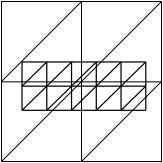
\includegraphics[width=0.95\linewidth]{pics/pdf/cube_bar_discretization.pdf} }
 	 	\end{minipage}
 
   \caption[Illustration of discretizations of the deformable bar on the rigid cube.]{Illustration of discretizations of the deformable bar on the rigid cube. In the center of the bar more features are overlapping than at the edging and thus there are more feature collisions.}
   \label{fig::defCubeVsBar}
 \end{figure}
 
 \begin{figure}[h!] 
 \begin{minipage}[b]{0.50 \linewidth}
 		\centering
 		\subfigure[Repulsion force with DPF ]{
        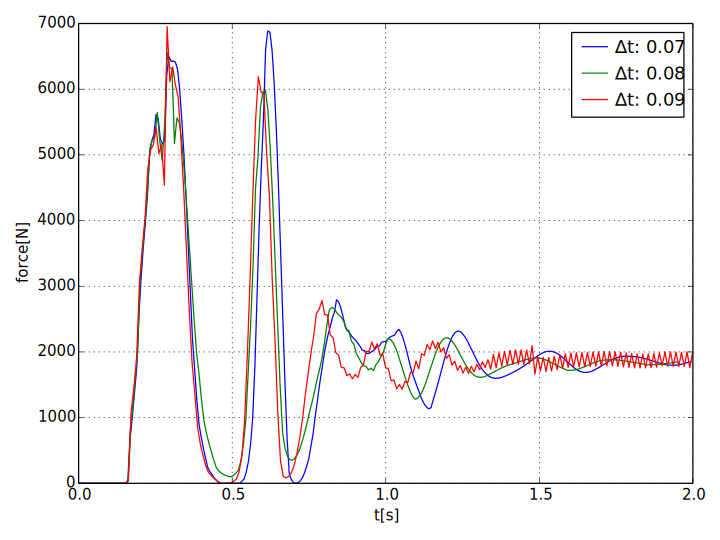
\includegraphics[width=1.0\linewidth]{pics/pdf/cubeBlockBM_dt_dpf.pdf} }
 	\end{minipage}
 	\begin{minipage}[b]{0.50 \linewidth}
 		\centering
 		\subfigure[Repulsion force with CPF]{
        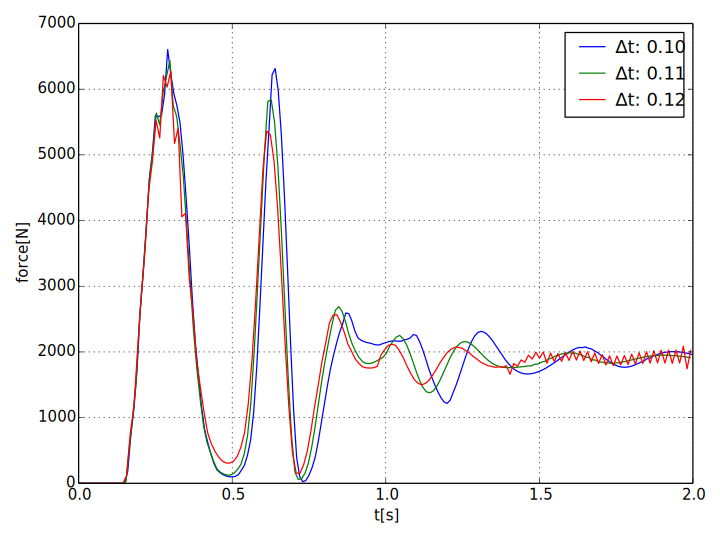
\includegraphics[width=1.0\linewidth]{pics/pdf/cubeBlockBM_dt_cpf.pdf} }
 	\end{minipage}
 \caption[Comparison of the repulsion force between a deformable bar and a rigid cube with varying time steps $\Delta t$ and and constant penalty coefficients $k=5000$.]{Comparison of the repulsion force between a deformable bar and a rigid cube with varying time steps $\Delta t$ and and constant penalty coefficients $k=5000$. The left plots show the force with DPF and jitter can be noted for $\Delta t=0.009$, whereas for the plots on right side with CPF jitter can be initially noted for a larger time step $\Delta t=0.012$}
 \label{fig::BlockBM_dt}
 \end{figure} 

We set the penalty coefficient to $k=5000$ and vary the time step sizes. % and examined the first to seconds whereupon the deformable bar rests on the rigid cube.
DPF resolve the collisions without notable jitter for time steps up to $\Delta t_d=0.08$, whereas CPF are smooth for time steps up to $\Delta t_c=0.11$. This matches roughly the ratio of 1.22 predicted in the particle-on-plane analysis.
The jitter observed in simulation is also notable in the plot of the collision forces between the cube and the bar as shown in figure \ref{fig::BlockBM_dt}.
Figure \ref{fig::BlockBM_dt} a) shows the DPF repulsion forces for time steps sizes $\Delta t=0.007s$, $\Delta t=0.008s=\Delta t_d$, $\Delta t=0.009s$ and figure \ref{fig::BlockBM_dt} b) shows the CPF repulsion forces for time steps sizes $\Delta t=0.010s$, $\Delta t=0.011s=\Delta t_c$, $\Delta t=0.012s$.
The overall plots are similar, there are two large peaks in the beginning at $t=0.3s$ and $t=0.6s$ with high repulsion forces when the deformable bar collides with the rigid cube and is pushed up again.
From $t\approx0.8s$ on the bar tumbles on the block, arising as a damped oscillation. There is a jitter notable in the force process for the higher time steps of each method.
For DPF, especially for $\Delta t=0.009$, it is notable from $t=0.7$ on and for CPF  it is notable for $\Delta t=0.012$ from $t=1.4$ on. This jitter in the force plot is also optically notable as jitter in the movement of vertices.
 

The jitter mainly takes place at the vertices in the middle of the bottom side of the bar, since there are more feature collisions than at the physical edges due to the discretization of the cube as shown in figure \ref{fig::defCubeVsBar} c).
In the center of the bar, more features overlap than at the physical edge and thus there are more feature collisions.\\
In sum we have seen that also for a more complex scenario CPF provide stability for larger time steps and validated the results from the particle-plane scenario.\\
Up to now the penalty coefficient was constant and we varied the time step.
In the following we vary both, the time step and the penalty coefficient to reach a comprehensive comparison of the CPF and DPF.\\
We chose multiple time steps $\Delta t$ and in order he provide stable simulations compute $k$ according to the relation $\Delta t \sim \sqrt{\frac{m}{k}}$ from the 1D particle analysis. 
The resulting forces are shown in figure \ref{fig::defBar_vs_RigCubeBM}.
For all four cases, CPF provide a much smoother force curve than the DPF. Again, it is also notable in the simulation since there is a notable jitter for DPF.\\ 
\begin{figure}[tp] 
\begin{minipage}[b]{0.5 \linewidth}
		\centering
		\subfigure[$\Delta$t=0.005, k=20000]{
			       \includegraphics[width=1.0\linewidth]{pics/pdf/cubeBM_t0005.pdf} }
	\end{minipage}
	\begin{minipage}[b]{0.5 \linewidth}
		\centering
		\subfigure[$\Delta$t=0.01, k=5000]{
			       \includegraphics[width=1.0\linewidth]{pics/pdf/cubeBM_t001.pdf} }
	\end{minipage}\\	
	\begin{minipage}[b]{0.5 \linewidth}
			\centering
			\subfigure[$\Delta$t=0.02, k=1250]{
				       \includegraphics[width=1.0\linewidth]{pics/pdf/cubeBM_t002.pdf} }
		\end{minipage}
		\begin{minipage}[b]{0.5 \linewidth}
			\centering
			\subfigure[$\Delta$t=0.04, k=500]{
				       \includegraphics[width=1.0\linewidth]{pics/pdf/cubeBM_t004.pdf} }
		\end{minipage}

  \caption{The repulsion force between a deformable bar and a rigid cube with varying time steps dt and penalty coefficients k.}
  \label{fig::defBar_vs_RigCubeBM}
\end{figure}
\begin{figure}[h] 
		\centering
			       \includegraphics[width=0.5\linewidth]{pics/pdf/defBar_vs_RigCubeBM_depth.pdf} 

  \caption[The average of the summed penetration depth per time step for a deformable bar dropped on a rigid cube with varying time steps an penalty coefficients.]{The average of the summed penetration depth per time step for a deformable bar dropped on a rigid cube with varying time steps and penalty coefficients. For increasing time steps the penalty coefficients decrease and accordingly the penetration depth increases. It is noticeable that the penetration depth with CPF is between 1.4 and 2.0 times higher than the penetration depth with DPF.}
  \label{fig::defBar_vs_RigCubeBM_depth}
\end{figure}
However, the summed penetration depth per time step, as shown in figure \ref{fig::defBar_vs_RigCubeBM_depth}, is for CPF  between 1.4 and 2.0 times larger than for DPF. The DPF algorithm yields larger collison forces due to the larger overestimation of the penetration depth while the intersection is increasing, as explained in section \ref{sec:CPFGENERAL}.

We have shown that the penetration depth for CPF is larger than for DPF with equal penalty coefficients, but for these cases the DPF were already jittering whereas CPF behaved smooth. In order to make a valid statement, we have to investigate the penetration depth and the jitter for varying penalty coefficients.

\begin{figure}[h!] 
\begin{minipage}[b]{0.5 \linewidth}
		\centering
		\subfigure[CPF]{
			       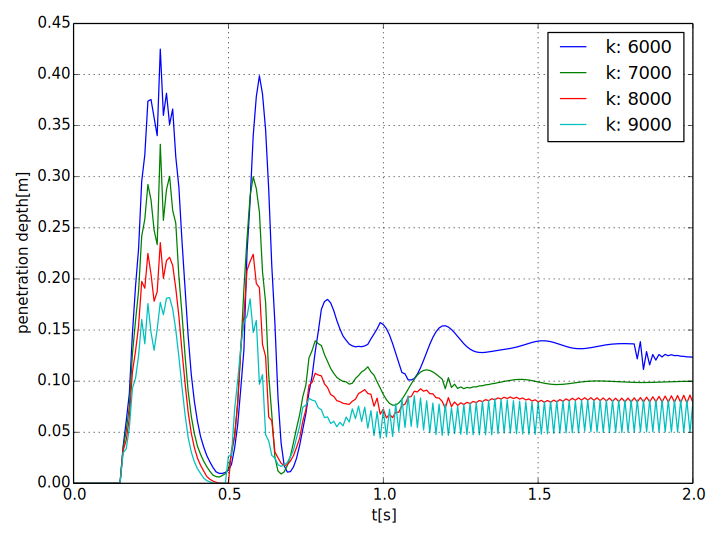
\includegraphics[width=1.0\linewidth]{pics/pdf/pendepth_cpf.pdf} }
	\end{minipage}
	\begin{minipage}[b]{0.5 \linewidth}
		\centering
		\subfigure[DPF]{
			       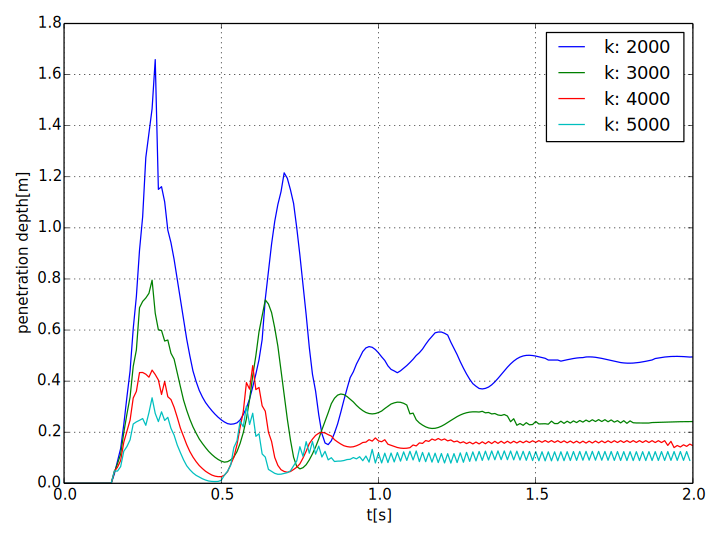
\includegraphics[width=1.0\linewidth]{pics/pdf/pendepth_dpf.pdf} }
	\end{minipage}
  \caption[The penetration depth for CPF and DPF with varying penalty coefficients and constant time step $\Delta t=0.01s$.]{The penetration depth for CPF and DPF with varying penalty coefficients and constant time step $\Delta t=0.01s$. (Note the different scaling of the y-axis and the different penalty coefficients). For the equilibrium, CPF provide smooth behavior up to k=8000 with a penetration depth of 0.1m, whereas DPF only provide an almost smooth behavior up to k=3000, with a penetration depth of 0.28m.}
  \label{fig::pendepth_comp}
\end{figure}

Again, we drop the deformable bar on the rigid cube, this time with a constant time step $\Delta t=0.01$ and varying penalty coefficients $k$. The penetration depths are shown in figure \ref{fig::pendepth_comp}.
For the equilibrium CPF, provide smooth behavior up to k=7000 with a penetration depth of 0.1m, whereas DPF only provide an almost smooth behavior up to $k=3000$, with a penetration depth of 0.28m.



In this section, we compared the CPF algorithm by Tang et al. \cite{TANG2012} to DPF and showed that for a constant penalty coefficient CPF can handle larger time steps without jitter. However, the DPF provide smaller penetration depths with an equal penalty coefficient. Nevertheless, with an increased penalty coefficient for the CPF, CPF are still stable and provide smaller intersections. In comparison, the DPF are with a smaller penalty coefficient already jittering and yield larger penetration depths.

In conclusion the CPF algorithm provides increased stability, less jitter and smaller penetration depths.

\section{Contact Redefinition}
\label{sec::res_redef}
To analyze the new approach of contact redefinition (described in section \ref{sec::CPFExtensions}) we simulate a rigid cube sliding on a deformable bar with and without the collision redefinition algorithm (see figures \ref{fig::redef_collsVFwo}- \ref{fig::redef_collsEE}). There is no friction applied, therefore the tangential motion should not change.

Without the redefinition algorithm the rigid cube changes its velocity in an implausible fashion tangential to the bar and bounces between the surface edges and vertices of the bar. It is hooked between the surface elements. The tangential forces are caused by the highlighted collisions in figure \ref{fig::redef_collsEEwo} (b)-(f) and \ref{fig::redef_collsVFwo} (f). Furthermore, there are implausible collisions in \ref{fig::redef_collsVFwo} (b)and (c). The highlighted vertices  \ref{fig::redef_collsVFwo} (b)and (c) would be expected to be colliding with the vertex of the face directly below and not with the neighboring face.
In contrast, with the redefinition algorithm (see figure  \ref{fig::redef_collsVF} and \ref{fig::redef_collsVF}) the cube's tangential velocity does not change notable, it slides on the bar and tips over the edge. There are no wrong collisions inducing strong tangential forces and no implausible collision pairs.

\begin{figure}[tbp] 
			\begin{minipage}[b]{0.3 \linewidth}
				\centering
				\subfigure[t=0.00s]{
					       \includegraphics[width=1.0\linewidth]{pics/png/redef_vf01wo.png} }
			\end{minipage}
			\begin{minipage}[b]{0.3 \linewidth}
				\centering
				\subfigure[t=0.50s]{
					       \includegraphics[width=1.0\linewidth]{pics/png/redef_vf02wo.png} }
			\end{minipage}
			\begin{minipage}[b]{0.3 \linewidth}
				\centering
				\subfigure[t=1.00s]{
		       \includegraphics[width=1.0\linewidth]{pics/png/redef_vf03wo.png} }
			\end{minipage}\\
			
				\begin{minipage}[b]{0.3 \linewidth}
					\centering
					\subfigure[t=1.50s]{
						       \includegraphics[width=1.0\linewidth]{pics/png/redef_vf04wo.png} }
				\end{minipage}
				\begin{minipage}[b]{0.3 \linewidth}
					\centering
					\subfigure[t=2.00s]{
						       \includegraphics[width=1.0\linewidth]{pics/png/redef_vf05wo.png} }
				\end{minipage}
				\begin{minipage}[b]{0.3 \linewidth}
					\centering
					\subfigure[t=2.50s]{
			       \includegraphics[width=1.0\linewidth]{pics/png/redef_vf06wo.png} }
				\end{minipage}\\
				\caption[A rigid cube sliding on a deformable bar without the collision redefinition algorithm and without friction.]{A rigid cube sliding on a deformable bar without the collision redefinition algorithm and without friction. The sideway collision pairs induce implausible tangential forces affecting the movement of the rigid cube in an implausible way.  The subfigures show active VF collisions, with the vertices in red and the faces in blue, the features inducing artifact forces are highlighted orange.}
				\label{fig::redef_collsVFwo}
\end{figure}

\begin{figure}[tbp] 
			\begin{minipage}[b]{0.3 \linewidth}
				\centering
				\subfigure[t=0.00s]{
					       \includegraphics[width=1.0\linewidth]{pics/png/redef_vf01.png} }
			\end{minipage}
			\begin{minipage}[b]{0.3 \linewidth}
				\centering
				\subfigure[t=0.50s]{
					       \includegraphics[width=1.0\linewidth]{pics/png/redef_vf02.png} }
			\end{minipage}
			\begin{minipage}[b]{0.3 \linewidth}
				\centering
				\subfigure[t=1.00s]{
		       \includegraphics[width=1.0\linewidth]{pics/png/redef_vf03.png} }
			\end{minipage}\\
			
				\begin{minipage}[b]{0.3 \linewidth}
					\centering
					\subfigure[t=1.50s]{
						       \includegraphics[width=1.0\linewidth]{pics/png/redef_vf04.png} }
				\end{minipage}
				\begin{minipage}[b]{0.3 \linewidth}
					\centering
					\subfigure[t=2.00s]{
						       \includegraphics[width=1.0\linewidth]{pics/png/redef_vf05.png} }
				\end{minipage}
				\begin{minipage}[b]{0.3 \linewidth}
					\centering
					\subfigure[t=2.50s]{
			       \includegraphics[width=1.0\linewidth]{pics/png/redef_vf06.png} }
				\end{minipage}\\
				\caption[A rigid cube sliding on a deformable bar with the collision redefinition algorithm and without friction.]{A rigid cube sliding on a deformable ba with the collision redefinition algorithm and without friction. With the redefinition algorithm no sideways collision appear and the cube slides plausible on the bar without notable changes in its tangential velocity. The subfigures show active VF collisions, with the vertices in red and the faces in blue.}
				\label{fig::redef_collsVF}
\end{figure}

\begin{figure}[tbp] 
	\begin{minipage}[b]{0.3 \linewidth}
		\centering
		\subfigure[t=0.00s]{
			       \includegraphics[width=1.0\linewidth]{pics/png/redef_ee01wo.png} }
	\end{minipage}
	\begin{minipage}[b]{0.3 \linewidth}
		\centering
		\subfigure[t=0.50s]{
			       \includegraphics[width=1.0\linewidth]{pics/png/redef_ee02wo.png} }
	\end{minipage}
	\begin{minipage}[b]{0.3 \linewidth}
		\centering
		\subfigure[t=1.00s]{
       \includegraphics[width=1.0\linewidth]{pics/png/redef_ee03wo.png} }
	\end{minipage}\\
	
		\begin{minipage}[b]{0.3 \linewidth}
			\centering
			\subfigure[t=1.50s]{
				       \includegraphics[width=1.0\linewidth]{pics/png/redef_ee04wo.png} }
		\end{minipage}
		\begin{minipage}[b]{0.3 \linewidth}
			\centering
			\subfigure[t=2.00s]{
				       \includegraphics[width=1.0\linewidth]{pics/png/redef_ee05wo.png} }
		\end{minipage}
		\begin{minipage}[b]{0.3 \linewidth}
			\centering
			\subfigure[t=2.50s]{
	       \includegraphics[width=1.0\linewidth]{pics/png/redef_ee06wo.png} }
		\end{minipage}
				\caption[A rigid cube sliding on a deformable bar without the collision redefinition algorithm and without friction.]{A rigid cube sliding on a deformable bar without the collision redefinition algorithm and without friction. The sideway collision pairs induce implausible tangential forces affecting the movement of the rigid cube in an implausible way. The subfigures show EE collisions in green and the collisions inducing implausible tangential forces are highlighted orange.}
				\label{fig::redef_collsEEwo}
\end{figure}

\begin{figure}[tbp] 
	\begin{minipage}[b]{0.3 \linewidth}
		\centering
		\subfigure[t=0.00s]{
			       \includegraphics[width=1.0\linewidth]{pics/png/redef_ee01.png} }
	\end{minipage}
	\begin{minipage}[b]{0.3 \linewidth}
		\centering
		\subfigure[t=0.50s]{
			       \includegraphics[width=1.0\linewidth]{pics/png/redef_ee02.png} }
	\end{minipage}
	\begin{minipage}[b]{0.3 \linewidth}
		\centering
		\subfigure[t=1.00s]{
       \includegraphics[width=1.0\linewidth]{pics/png/redef_ee03.png} }
	\end{minipage}\\
	
		\begin{minipage}[b]{0.3 \linewidth}
			\centering
			\subfigure[t=1.50s]{
				       \includegraphics[width=1.0\linewidth]{pics/png/redef_ee04.png} }
		\end{minipage}
		\begin{minipage}[b]{0.3 \linewidth}
			\centering
			\subfigure[t=2.00s]{
				       \includegraphics[width=1.0\linewidth]{pics/png/redef_ee05.png} }
		\end{minipage}
		\begin{minipage}[b]{0.3 \linewidth}
			\centering
			\subfigure[t=2.50s]{
	       \includegraphics[width=1.0\linewidth]{pics/png/redef_ee06.png} }
		\end{minipage}
				\caption[A rigid cube sliding on a deformable barwith the collision redefinition algorithm and without friction.]{A rigid cube sliding on a deformable bar with the collision redefinition algorithm and without friction. With the redefinition algorithm no sideways collision appear and the cube slides plausible on the bar without notable changes in its tangential velocity. The subfigures show active EE collisions in green and candidate collisions in red.}
				\label{fig::redef_collsEE}
\end{figure}

The repulsion forces are shown in figure \ref{fig::force_redef}. The plot shows a smooth with several leaps. The leaps are induced by the contact redefinitions. When a sliding contact is redefined, there is a sudden additional geometrically deep collision providing a sudden increase of the contact force. Similarly, if an EE collision is added or removed by the redefinition algorithm, force changes are induced. Overall, these leaps are small and do not induce a notable jitter.

\begin{figure}[tbp]
\centering
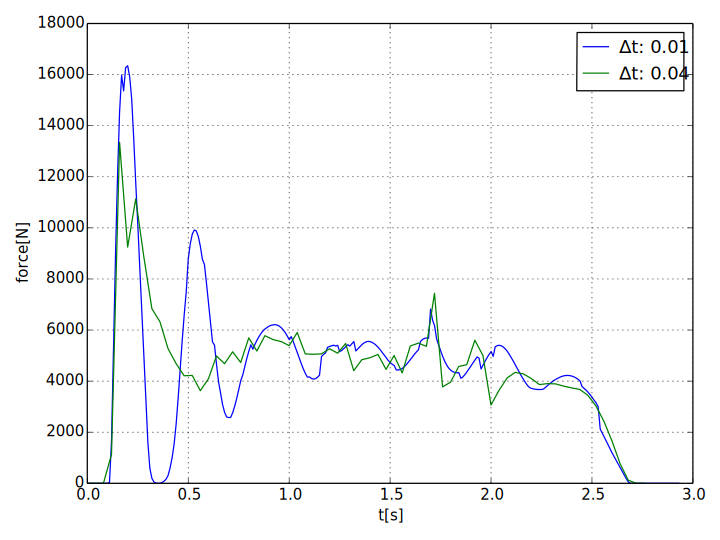
\includegraphics[width=0.60\linewidth]{pics/pdf/slidingCube_redef_dt.pdf} 
\caption{Contact force for a rigid cube sliding on a deformable bar}
\label{fig::force_redef}
\end{figure}
\begin{figure}[tbp] 
	\begin{minipage}[b]{0.33 \linewidth}
		\centering
		\subfigure[t=0.00s]{
			       \includegraphics[width=0.97\linewidth]{pics/png/bunny01.png} }
	\end{minipage}
	\begin{minipage}[b]{0.33 \linewidth}
		\centering
		\subfigure[t=0.50s]{
			       \includegraphics[width=0.97\linewidth]{pics/png/bunny02.png} }
	\end{minipage}
	\begin{minipage}[b]{0.33 \linewidth}
		\centering
		\subfigure[t=1.00s]{
       \includegraphics[width=0.97\linewidth]{pics/png/bunny03.png} }
	\end{minipage}\\
	
		\begin{minipage}[b]{0.33 \linewidth}
			\centering
			\subfigure[t=1.50s]{
				       \includegraphics[width=0.97\linewidth]{pics/png/bunny04.png} }
		\end{minipage}
		\begin{minipage}[b]{0.33 \linewidth}
			\centering
			\subfigure[t=2.00s]{
				       \includegraphics[width=0.97\linewidth]{pics/png/bunny05.png} }
		\end{minipage}
		\begin{minipage}[b]{0.33 \linewidth}
			\centering
			\subfigure[t=2.50s]{
	       \includegraphics[width=0.97\linewidth]{pics/png/bunny06.png} }
		\end{minipage}
				\caption{A deformable bunny is dropped in a rigid bowl, which is dropped on a static plane.}
				\label{fig::bunnyBowl}
\end{figure}

\begin{figure}[tbp]
		\centering
			       \includegraphics[width=0.4\linewidth]{pics/png/bunny_inverted.png} 
	
\caption{Inverted tetrahedrons (marked red) occur when the deformable bunny collides with the rigid bowl.}
\label{fig::bunny_inverted}
\end{figure}

Up to now we analyzed rather simple geometries. Therefore, we will now investigate a more complex scene, with a bunny dropped in a rigid bowl with CPF and the redefinition algorithm. Screenshots of the simulation are shown in figure \ref{fig::bunnyBowl}.

The bunny drops in the bowl, bounces around for approximately two seconds and then comes to rest. The overall result is visually satisfying. However, a closer look at the bunny shows that when it is colliding some tetrahedrons are inverted , see figure \ref{fig::bunny_inverted}. Inverted tetrahedrons disturb the visual impression of the scene. They are induced due to large collision impulses by the CPF algorithm and can be reduced by choosing lower penalty coefficients. Nevertheless, reducing the penalty coefficients yields larger penetration depths.
\newpage

To sum it up, we have shown in the cube-bar benchmark that the redefinition algorithm provides plausible collision pairs and preserves the tangential motion, whereas with the original CPF algorithm we obtained an implausible stop of the tangential motion. Furthermore, we proved that the redefinition algorithm can handle complex geometries, as shown in the bunny-bowl scene.

\section{Friction}
To achieve a plausible friction behavior, the friction model should induce forces according to Coulombs law. Dynamic friction should slow down the tangential movement. Static friction should stop any tangential movement if the tangential velocity is close to zero and the tangential force $\mathbf f_t$ is smaller than the product of the static friction coefficient $\mu_S $ and the normal force $\mathbf f_n$.


To analyze the friction model, we investigate a rigid cube with mass $m=100kg$ sliding on a $10^\circ$ slope. To test the static friction, the velocity of the rigid cube is initialized with $v_0=3\frac{m}{s}$ upwards the plane. We used continuous penalty forces with a penalty coefficient $k=20000$. The dynamic friction coefficient is set to $\mu_d=0.1$ and the static friction is set to $\mu_s=0.3$ and $\mu_s=0.4$. The friction penalty coefficients are set to $k_{fp}=100$, $k_{fd}=25$ and $k_f=10000$.

\begin{figure}[h!]
	\begin{minipage}[b]{0.5 \linewidth}
		\centering
		\subfigure[static friction coefficients $\mu_s=0.3$]{
			       \includegraphics[width=1.0\linewidth]{pics/pdf/block_fric_dyn.pdf} }
	\end{minipage}
	\begin{minipage}[b]{0.5 \linewidth}
		\centering
		\subfigure[static friction coefficients $\mu_s=0.4$]{
			       \includegraphics[width=1.0\linewidth]{pics/pdf/block_fric_stat.pdf} }
	\end{minipage}	
\caption[Position and velocity over time of a rigid cube sliding on a slope with different static friction coefficients $\mu_s$.]{Position and velocity over time of a rigid cube sliding on a slope with different static friction coefficients $\mu_s$. With the lower coefficient $\mu_s=0.3$ the cube slides up the slope until its velocity reaches zero, then it starts sliding down. Whereas, with the higher coefficient $\mu_s$ the cube stops after its velocity reached zero and stays at its position.}
\label{fig::friction_dynstat}
\end{figure}

The movement and the velocity of the cube are shown in figure \ref{fig::friction_dynstat}.
For the lower coefficient $\mu_s=0.3$ the cube slides up the plane with decreasing velocity, decelerated by gravity and dynamic friction.
At $t\approx 1.2s$ it reaches the maximum height and starts sliding down again with increasing velocity, this time accelerated by gravity and slightly decelerated by dynamic friction.

For the higher coefficient $\mu_s=0.4$ the cube starts exactly equal to the previous one. However, when it reaches the top it remains at the position, due to the increased static friction coefficient. The static friction is now larger than the	downhill-slope force. The velocity shows a small damped oscillation at $t\approx 1.2s$, it is induced since we model the static friction by applying a damped spring at the point where the cube is to be hold.

Comparing the results with the analytical solution of Coulomb's Friction law, we would expect the block to stop for $\mu_s>0.176$, whereas in our simulation the block stopped for $\mu_s \gtrsim 0.4$. Nevertheless the friction model provides  results analogously to Coulomb's Friction law, providing satisfying results for an interactive environment.

To analyze the friction between multiple bodies we place a rigid cube with an initial velocity on a deformable bar and simulate two different friction coefficients. Furthermore, to test for numerical drift in the position due to the static friction we will analyze the simulation for a large number of time steps (20000).

\begin{figure}[h!]
	\begin{minipage}[b]{0.5 \linewidth}
		\centering
		\subfigure[$\mu_s=0.8$, $\mu_d=0.1$, $t=0.2s$]{
			       \includegraphics[width=1.0\linewidth]{pics/png/sliding_block_mus08_md01_a.png} }
	\end{minipage}
	\begin{minipage}[b]{0.5 \linewidth}
		\centering
		\subfigure[$\mu_s=0.8$, $\mu_d=0.1$, $t=20.0s$]{
			       \includegraphics[width=1.0\linewidth]{pics/png/sliding_block_mus08_md01_b.png} }
	\end{minipage}\\
	
		\begin{minipage}[b]{0.5 \linewidth}
			\centering
			\subfigure[$\mu_s=0.3$, $\mu_d=0.05$, $t=0.35s$]{
				       \includegraphics[width=1.0\linewidth]{pics/png/sliding_block_mus03_md005_a.png} }
		\end{minipage}
		\begin{minipage}[b]{0.5 \linewidth}
			\centering
			\subfigure[$\mu_s=0.3$, $\mu_d=0.05$, $t=20.0s$]{
				       \includegraphics[width=1.0\linewidth]{pics/png/sliding_block_mus03_md005_b.png} }
		\end{minipage}		
\caption[A rigid cube sliding from the right to the left on a deformable bar with two friction coefficient combinations.]{A rigid cube sliding from the right to the left on a deformable bar with two friction coefficient combinations. (a) and (c) show the cube right after the static friction set in. (b) and (d) show the cube after two seconds. With the lower valued coefficient combination the cube keeps sliding further than with higher combination due to dynamic friction. After the blocks stopped they rest at their position due to static friction.}
\label{fig::block_sliding_fric_longtime}
\end{figure}

Screenshots of the scene are shown in figure \ref{fig::block_sliding_fric_longtime}. The cube starts at the right side with its initial velocity in the left direction. With the higher friction coefficients in a) and b) the cube is stronger decelerated as with the lower coefficients in c) and d).
After the cube stopped it movements (a) and c), it rests exactly at its position. Even after 20000 steps there is no numerical drift in the position notable. This a result of the static friction modeled with a fixed spring. Therefore the bodies can make small movements around the fixed position, but no optically notable movement or position drift is possible.

In conclusion the penalty-based friction model \cite{YAMANE2006} applies a plausible modeling of dynamic and static friction with no notable numerical drift in the position for the static friction.
The model does not grant the analytical description of Coulomb's friction law. However it provides analogue results, which are satisfying for the use in an interactive environment.


\section{Computational Cost}
\label{sec:compCost}
The computational cost is a crucial property for interactive applications. Therefore, we investigate the computational cost of the CPF in comparison to the DPF with regard to the results from the stability analysis.
 
We analyzed the scene with a deformable bunny dropped into a rigid bowl from section \ref{sec::res_redef} (see figure \ref{fig::bunnyBowl}) using an Intel Core i7-2630QM 2.0Ghz processor with 6.0GB RAM and a Nvidia Geforce 540M graphics card.
To provide an accurate comparison of the CPF and DPF, we simulate the scene with CPF and compute for each feature pair the impulse with both algorithms, though DPF computation is only for time measurements and the impulses are not applied.
We measured five runs with 200 simulation steps each and detecting the time for the handling of each feature and its components.
The averaged times are shown in figure \ref{fig::compCost_scene}.

\begin{figure}[h]
		\centering
			       \includegraphics[width=0.9\linewidth]{pics/pdf/comparison_comptime_cpf_dpf.pdf} 	
\caption{Composition of the computation time for one feature pair}
\label{fig::compCost_scene}
\end{figure}
The handling for a single EE pair takes average $6.8\mu s$, whereas a VF pair is slightly slower and takes average $7.8 \mu s$. The difference is mainly caused by the overall most expensive part of the collision handling, the categorization of the collision. For the EE pair, the collision categorization takes average $3.11 \mu s$ and thereby $45.7\%$ of the overall time for one feature pair. In the VF case, the categorization takes average $4.07\mu s$ and thereby $53.1 \%$ of the overall time for one feature pair.
The difference in the computation time of the VF and EE categorization can be explained by examining the number of tested normals. 
A vertex is typically adjacent to six faces and accordingly six normals need to be tested. Whereas, in the EE categorization each edge has only two directly adjacent faces, yielding only four normals to be tested. In sum, there are to more tests for the VF case and consequently the VF categorization is more expensive.
All other parts take almost the same time for VF and EE.
It is remarkable that the actual impulse computation in the VF case with CPF takes only  $12.9 \%$ (EE $14.6\%$) of the overall computation time and for DPF only $3.7\%$ (EE $4.1\%$).


A comparison of the computation time for one impulse with CPF and DPF is shown in figure \ref{fig::comparison_comptime_cpf_dpf_imp}.
The computation of the impulse with CPF takes in the VF case $1,01 \mu s$ (EE $1.00 \mu s$) and for DPF in the VF case it takes $0,29 \mu s$ (EE $0.28 \mu s$). Hence, the DPF need only a third of the time the CPF need for the computation of one impulse. The computational overhead of the CPF seems reasonable, since the CPF require the computation of degree-six polynomial, whereas the DPF correspond to a linear polynomial.
\begin{figure}[tbp]
		\centering
			       \includegraphics[width=0.9\linewidth]{pics/pdf/comparison_comptime_cpf_dpf_imp.pdf} 
	
\caption{Comparison of the computation time for one impulse with CPF and DPF}
\label{fig::comparison_comptime_cpf_dpf_imp}
\end{figure}
However, the impulse computation is only one component in the handling of a collision. In order gain a valid statement, we need to compare the overall computation time for a feature with DPF and CPF. With DPF the handling of one feature pair takes $6.83 \mu s$ (EE $5.84 \mu s$), whereas it takes $7.55 \mu s$ (EE $6.56 \mu s$) with CPF. The handling with CPF takes $11.8\%$ longer than the handling with DPF.
In section \ref{sec::stability} we have shown that the maximum time step for CPF is 1.22 times larger than for DPF. Combining the computational overhead with increased step size yields a theoretical speed-up of $9.12 \%$ for CPF. However, this result provides only limited validity, since DPF require only a DCD, whereas CPF require a CCD. In general, CCD provides a higher computational cost than DCD.

To compare the computational cost of DPF with a state of the art DCD to the computational cost of CPF with a state of the art CCD would yield an interesting and meaningful result in order to evaluate the actual difference in computational cost. However, the CCD in our framework is in a prototype state and far from optimal speed. Therefore, we cannot provide this analysis. However, Tang et al. \cite{TANG2012} compared DPF+DCD to CPF+CCD and showed that CPF+CCD are about 3 - 4 times slower than DPF+DCD.

In conclusion, the redefinition algorithm provides a significant additional cost by almost doubling the time needed to handle one collision pair. However, the additional cost is necessary in order to reduce the CPF artifacts, since otherwise no simulation of sliding contacts is feasible. The additional cost induced by the CPF in comparison to the DPF is small ($+11,8 \%$). However, CPF require CCD. Taking the collision detection into account and comparing the CCD+CPF to DCD+DPF shows that CPF+CCD are about 3 - 4 times slower than DPF+DCD \cite{TANG2012}.